\chapter{Getting Girls Involved}
In some parts of the country, getting girls to speak up in the classroom can be a real challenge.  Community culture, family upbringing, and previous experiences in the classroom can cause girls to ``feel shame" speaking aloud and thus do not take an active role in learning.  Over 50\% of Tanzanian girls aged 15 to 19 are married and only 25\% of girls in Tanzania have reached Standard 5. This statistics may seem overwhelming, however, getting girls involved in the classroom is one of the best ways to build their confidence and encourage empowerment in other areas of their life.  Try some of these tips in the classroom to encourage your female students.

\begin{itemize}
 \item Make a competition between boys and girls for participation points.  Every time a student tries to answer a question or read aloud, award them a point.  
 \item Call on boys and girls evenly.  Trying alternating between the two when having students answer questions.
 \item Use examples that relate to both genders.
 \item During group work, always make girls the leader, presenter, or writer to keep them actively engaged.
 \item Bring in strong female role models as guest speakers for different topics when teaching.
 \item Use confidence girls as examples other students. Reward girls when they speak up or participate in a school competition.
 \item Reward the highest scoring boy and girl for your tests.
 \item Make sure there is always a gender balance when doing debates, cleaning, or other school activities.
 \item Start a girls' football team, a stereotypically male sport in Tanzania.
 \item Start a girls' group after school.
 \item If girls speaking aloud is still a big problem, try separating streams by gender.  Build girls confidence together, then reintegrate them into a coed environment the following year.  
\end{itemize}

\begin{center}
\setlength\fboxsep{0pt}
\setlength\fboxrule{2pt}
\fbox{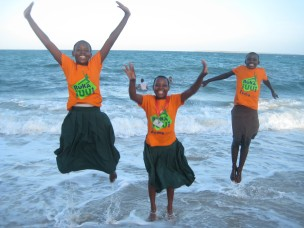
\includegraphics[scale=1]{./img/IMG_4778.JPG}}
\end{center}